\section{Experiments} \label{sec:experiments}

We now present the empirical evaluation of these coresets.
We ran two kinds of experiments. On real-world data sets, we merely computed a coreset $\Omega$, followed by running $k$-means++ on $\Omega$. 
The $k$-means++ algorithm was repeated 5 times, each yielding a solution $\calS_i$, and as the best lower bound on the distortion we used the largest ratio $\max_i\left(\max\left(\frac{\cost_A(\calS_i)}{\cost_{\Omega}(\calS_i)},\frac{\cost_{\Omega}(\calS_i)}{\cost_A(\calS_i)}\right)\right)$.
For the benchmark, we used the evaluation as proposed in Section~\ref{sec:benchmark}. In addition, we also determined the distortion via simply running the $k$-means++ algorithm. 

Except for BICO, which is deterministic, this experiment was repeated for each coreset algorithm $10$ times. \omar{Experiments were repeated 10 times including BICO. Although vanilla BICO is deterministic, we used BICO with heuristic speed optimizations which are stochastic.} We aggregated the reported distortions by taking the maximum over all $10$ evaluations. In addition, we also preprocessed the data using the dimension reduction techniques described in Section~\ref{sec:algorithms}.


\subsection{Datasets}
We use three common real-world datasets for evaluating $k$-means coresets 
---
\textit{Census}\footnote{\url{https://archive.ics.uci.edu/ml/datasets/US+Census+Data+(1990)}},
\textit{Covertype}\footnote{\url{https://archive.ics.uci.edu/ml/datasets/covertype}}, and 
\textit{Tower}\footnote{\url{http://homepages.uni-paderborn.de/frahling/coremeans.html}}
---
and several instances of the proposed benchmark. 
The \textit{Census} dataset is a small subset of the Public Use Microdata Samples from 1990 US census. It consists of demographic information encoded as 68 categorical attributes of 2,458,285 individuals. \textit{Covertype} is comprised of cartographic descriptions and forest cover type of four wilderness areas in the Roosevelt National Forest of Northern Colorado in the US. It consists of 581,012 records, 54 cartographic variables and one class variable. Although \textit{Covertype} was originally made for classification tasks, it is often used for clustering tasks by removing the class variable~\cite{AckermannMRSLS12}. \textit{Tower} is a 2,560 by 1,920 picture of a tower on a hill where each pixel is represented by a RGB color value. This dataset consists of 4,915,200 rows and 3 columns. To evaluate how denoising effects the quality of the output, we apply SVD\jesper{Should "SVD" be spelled out? I cannot find it anywhere in the paper. Is it a well known term?} on \textit{Census} and \textit{Covertype} using the $k$ largest singular values. Note that we do not reduce the number of dimensions of the original datasets. As for the benchmark dataset, instances are generated to match roughly the sizes of the real-world datasets. The chosen parameters values and the corresponding dataset sizes are shown in ~\cref{tab:benchmark-instances-overview}. 
% We generated a set of instances with no scaling i.e., $\beta=1.0$ (referred to as \textit{Benchmark-1.0}) and with maximum scaling; $\beta = 2.0$ (\textit{Benchmark-2.0}).




%
\begin{table}
	\begin{center}%\centering
	\caption{The sizes of the real-world datasets used for the experimental evaluation}
	\label{tab:real-world-datasets-overview}
% 	\resizebox{\textwidth}{!}{
	\begin{tabular}{lrr}
		\toprule
        
		    & Data points
		    & Dimensions
            \\
		\midrule
		\textit{Census}
    		& 2,458,285
    		& 68
    		\\
	    \textit{Covertype}
    	    & 581,012
    		& 54
    		\\
        \textit{Tover}
            & 4,915,200
    		& 3
    		\\
		\bottomrule
	\end{tabular}\\
	\end{center}
% 	}
\end{table}



%
\begin{table}
	\begin{center}%\centering
	\caption{The parameter values and the sizes of the benchmark instances used for the experimental evaluation.}
	\label{tab:benchmark-instances-overview}
% 	\resizebox{\textwidth}{!}{
	\begin{tabular}{rrrr}
		\toprule
        $k$
		    & $\alpha$
		    & Data points
		    & Dimensions
            \\
		\midrule
        10
    		& 6
    		& 1,000,000
    		& 60
    		\\
        20
    		& 5
    		& 3,200,000
    		& 100
    		\\
        30
    		& 4
    		& 810,000
    		& 120
    		\\
        40
    		& 4
    		& 2,560,000
    		& 160
    		\\
    %     50
    % 		& 4
    % 		& 6,250,000
    % 		& 200
    % 		\\
		\bottomrule
	\end{tabular}\\
	\end{center}
% 	}
\end{table}

\subsection{Algorithm Parameters}
We followed the same experimental procedure with respect to the choice of parameter values for the algorithms as prior works~\cite{AckermannMRSLS12, FGSSS13}. For the target coreset size, we used $200k$ for all our experiments. On \textit{Census} and \textit{Covertype}, we used $k$ values $\{10, 20, 30, 40, 50\}$, while for \textit{Tower} we used larger cluster sizes $k \in \{20, 40, 60, 80, 100\}$. On the benchmark instances, we settled on $k \in \{10, 20, 30, 40\}$ as a reasonable trade-off between running time and dataset size.



\subsection{Setup}
We implemented Sensitivity Sampling, Group Sampling and StreamKM++ in C++17 using Boost and Blaze libraries. The source code can be found on GitHub\footnote{Link to repository will be provided later.}. For BICO, we used the authors' reference implementation\footnote{\url{https://ls2-www.cs.tu-dortmund.de/grav/en/bico}}. The source code was compiled with gcc 9.3.0.
The experiments were performed on an Intel i7 machine (8 core, 3.4 GHz and 32 GB RAM) and an Intel i9 server (14 core, 3.3 GHz and 256 GB RAM).

\subsection{Results}

\begin{figure*}
  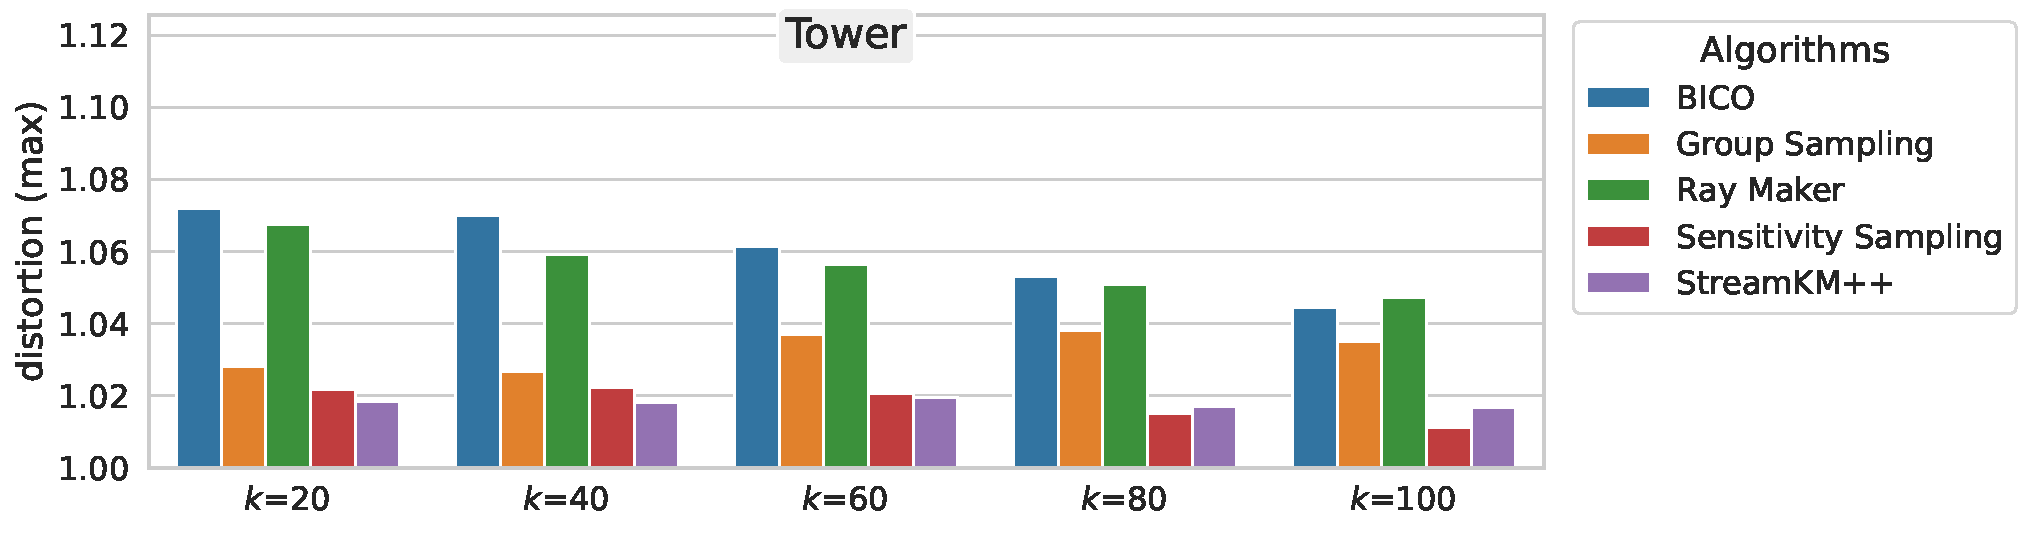
\includegraphics[width=.65\linewidth]{figures/distortions-Tower.pdf}
  \newline \newline
  \subfloat{
    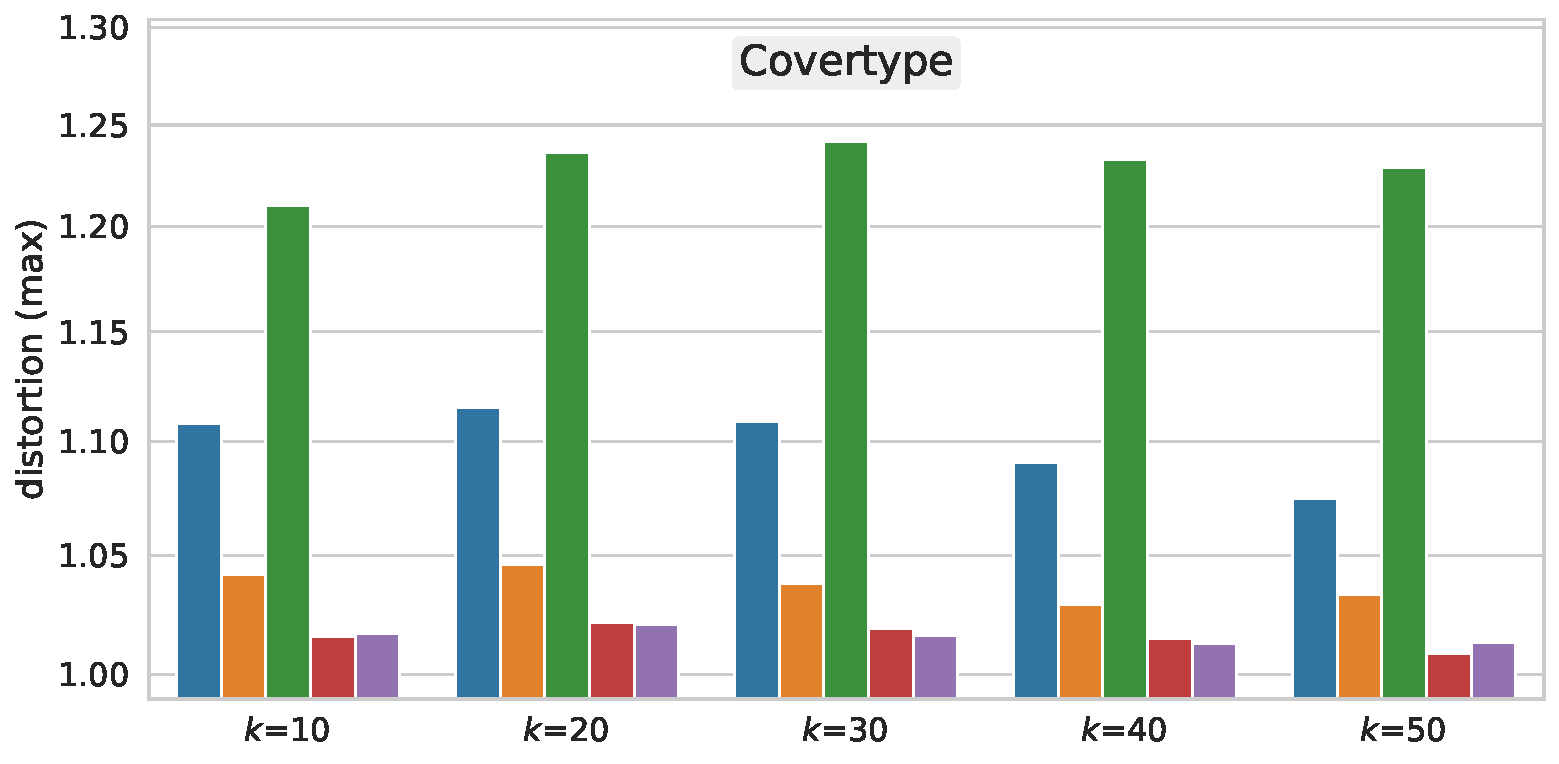
\includegraphics[width=0.5\textwidth]{figures/distortions-Covertype.pdf}
  }
  \subfloat{
    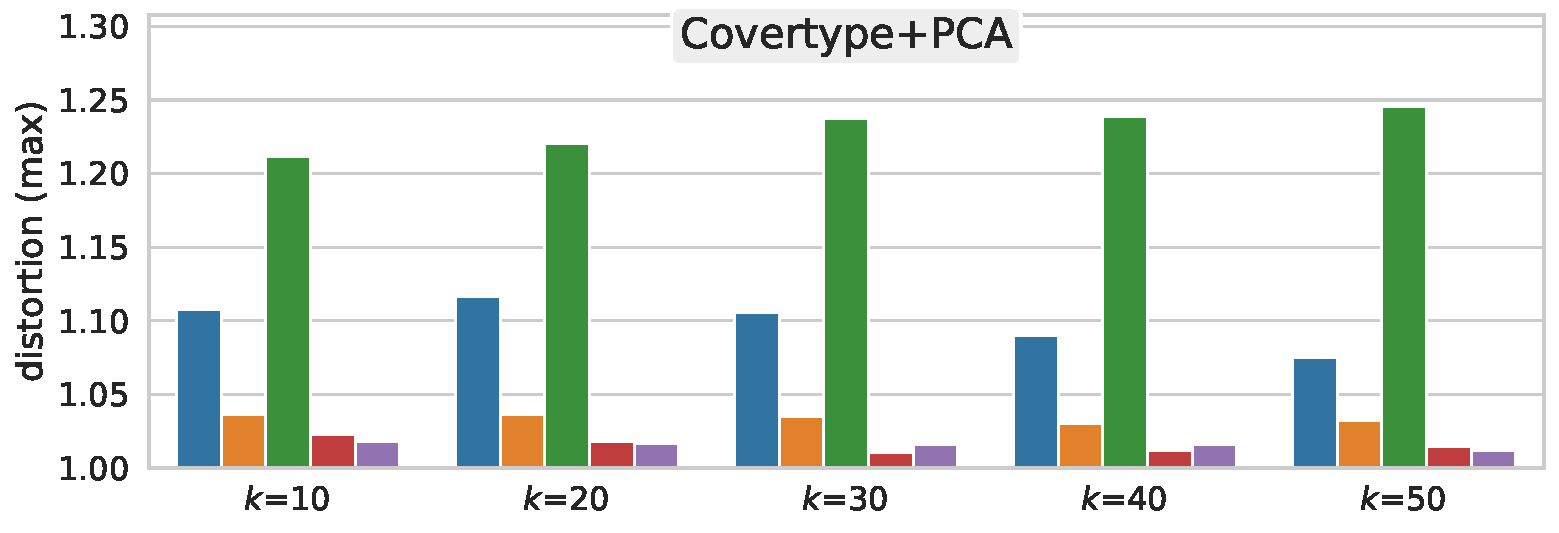
\includegraphics[width=.5\linewidth]{figures/distortions-Covertype+PCA.pdf}
  }
  \newline \newline
  \subfloat{
    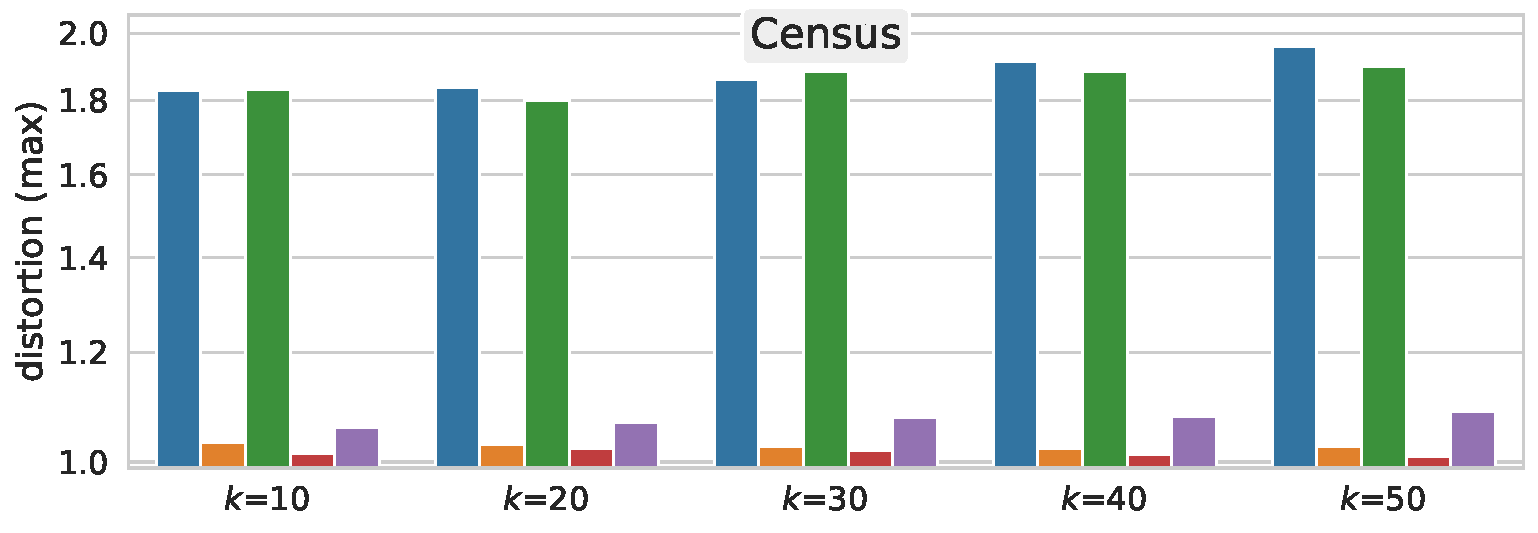
\includegraphics[width=0.5\textwidth]{figures/distortions-Census.pdf}
  }
  \subfloat{
    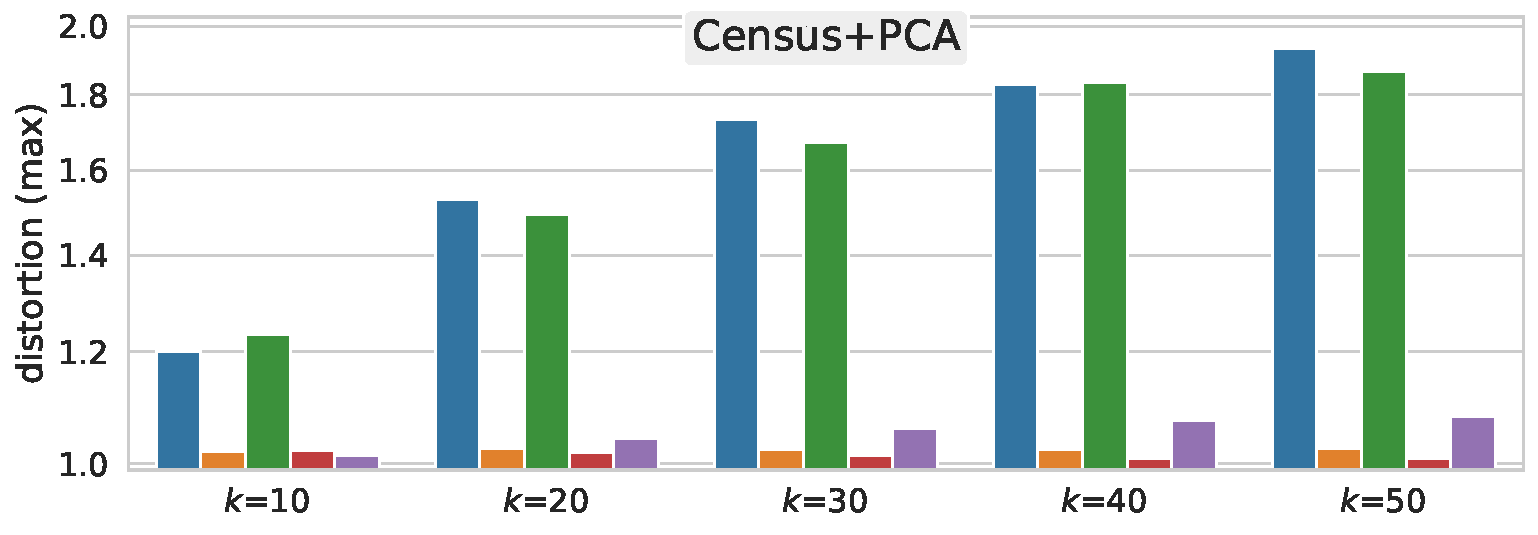
\includegraphics[width=.5\linewidth]{figures/distortions-Census+PCA.pdf}
  }
  \newline \newline
  \subfloat{
    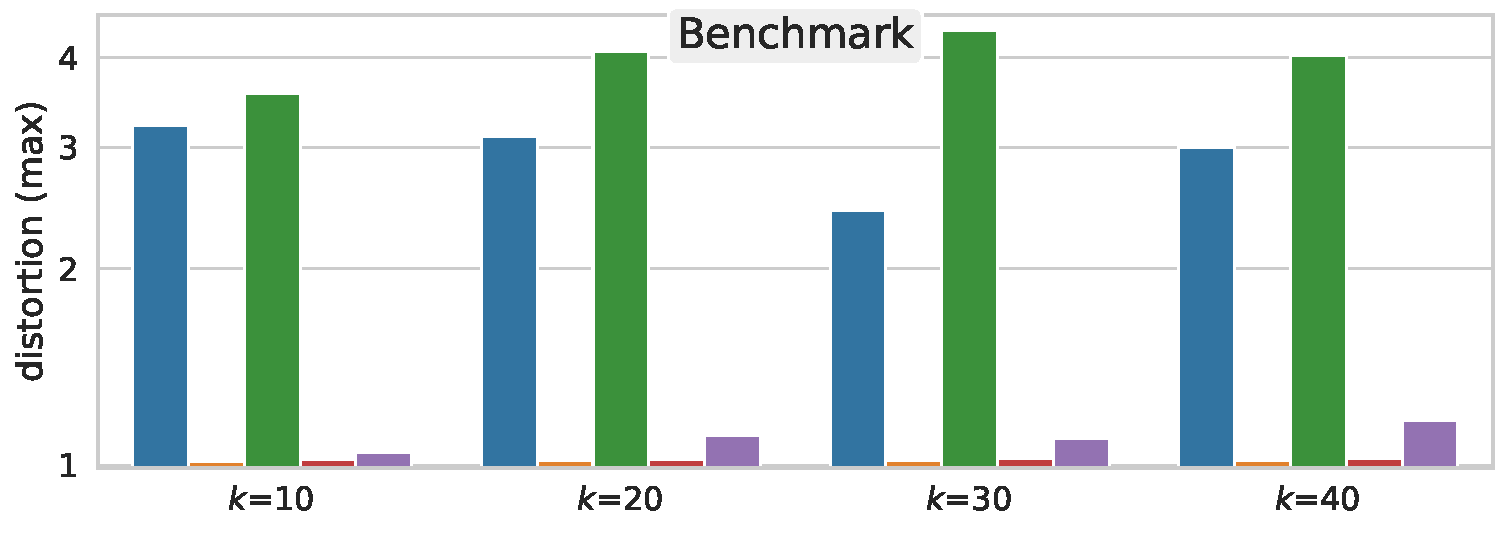
\includegraphics[width=0.5\textwidth]{figures/distortions-Benchmark.pdf}
  }
%   \subfloat{
%     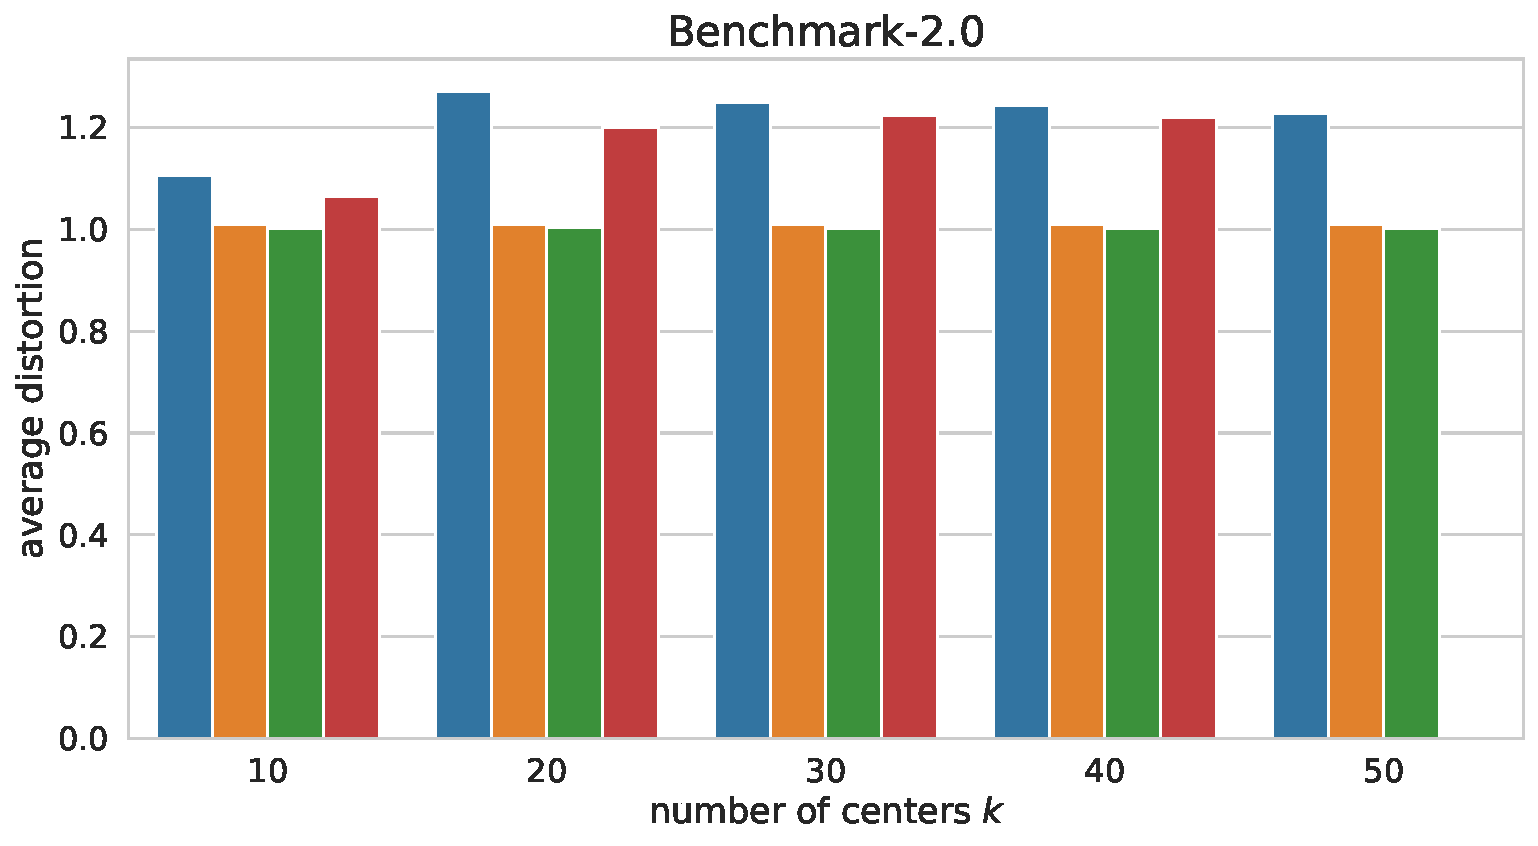
\includegraphics[width=.5\linewidth]{figures/results-Benchmark-2.0.pdf}
%   }
  \label{fig:results}
  \caption{The average distortion of the evaluated algorithms on different datasets.}
\end{figure*}




\begin{figure*}
  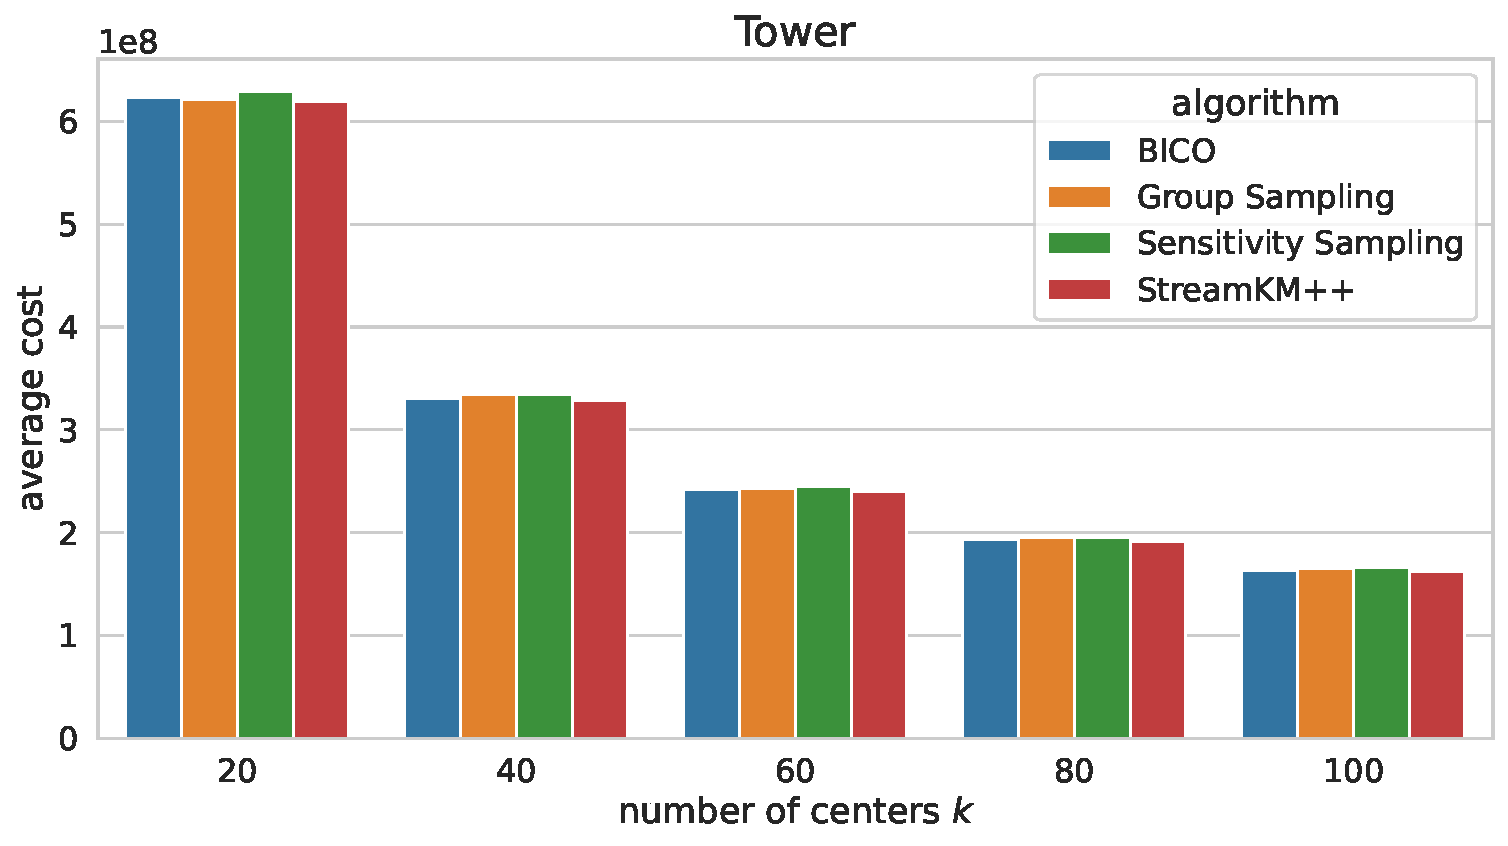
\includegraphics[width=.5\linewidth]{figures/costs-Tower.pdf}
  \newline \newline
  \subfloat{
    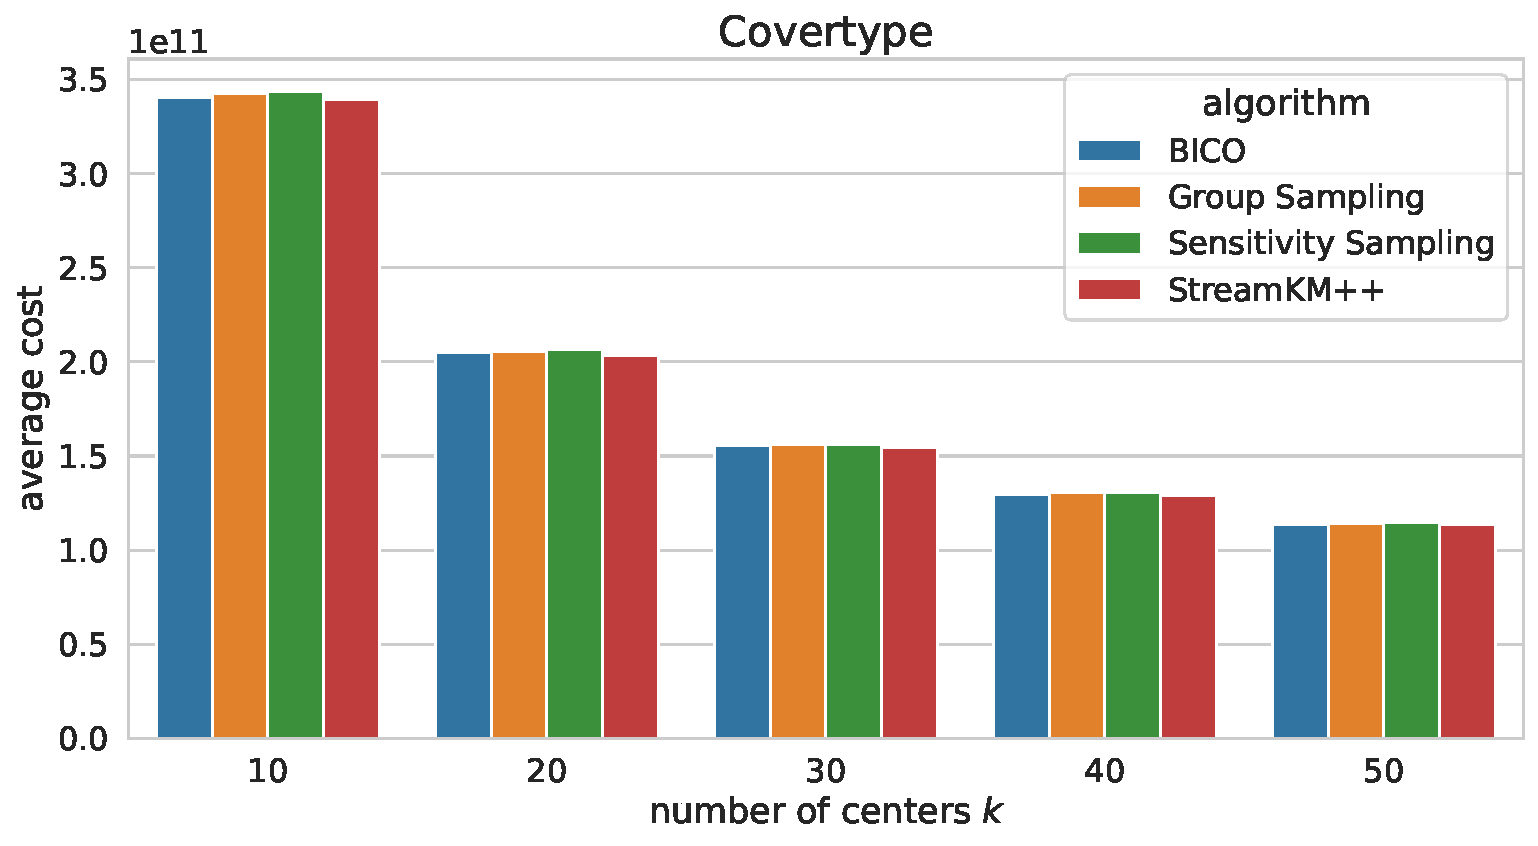
\includegraphics[width=0.5\textwidth]{figures/costs-Covertype.pdf}
  }
  \subfloat{
    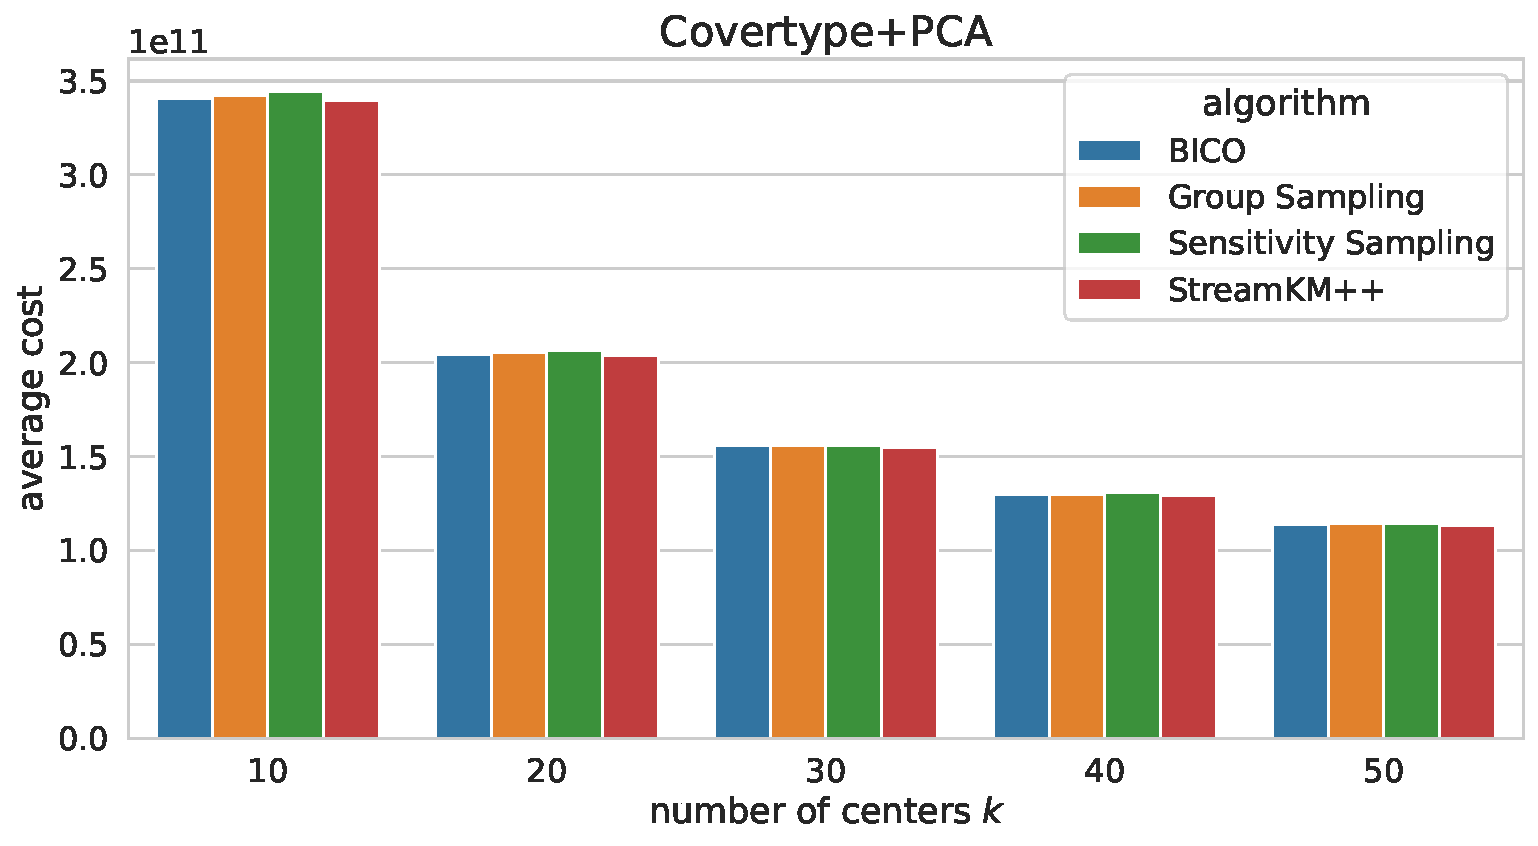
\includegraphics[width=.5\linewidth]{figures/costs-Covertype+PCA.pdf}
  }
  \newline \newline
  \subfloat{
    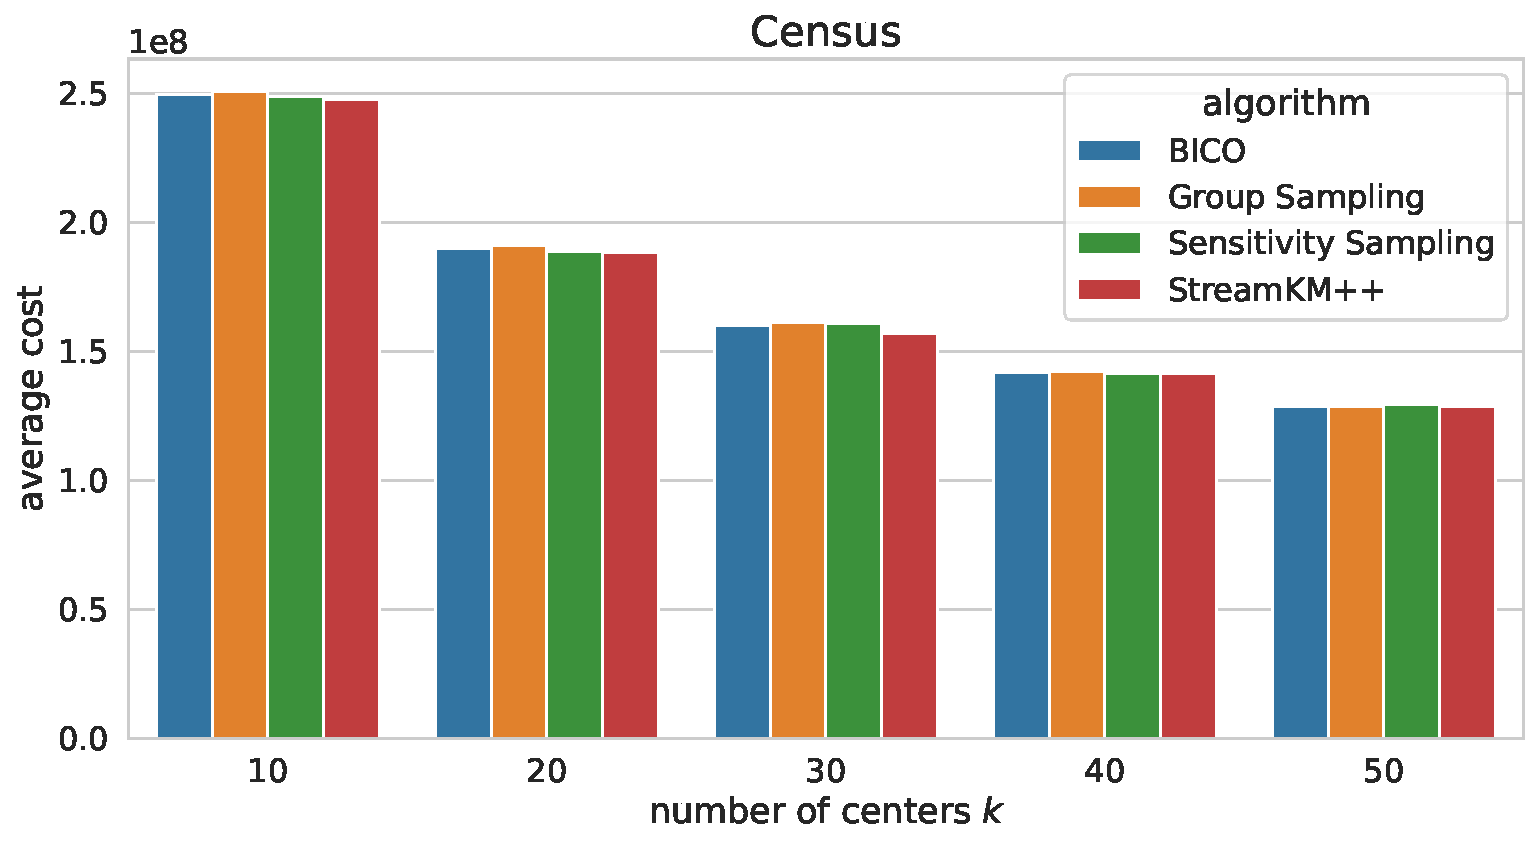
\includegraphics[width=0.5\textwidth]{figures/costs-Census.pdf}
  }
  \subfloat{
    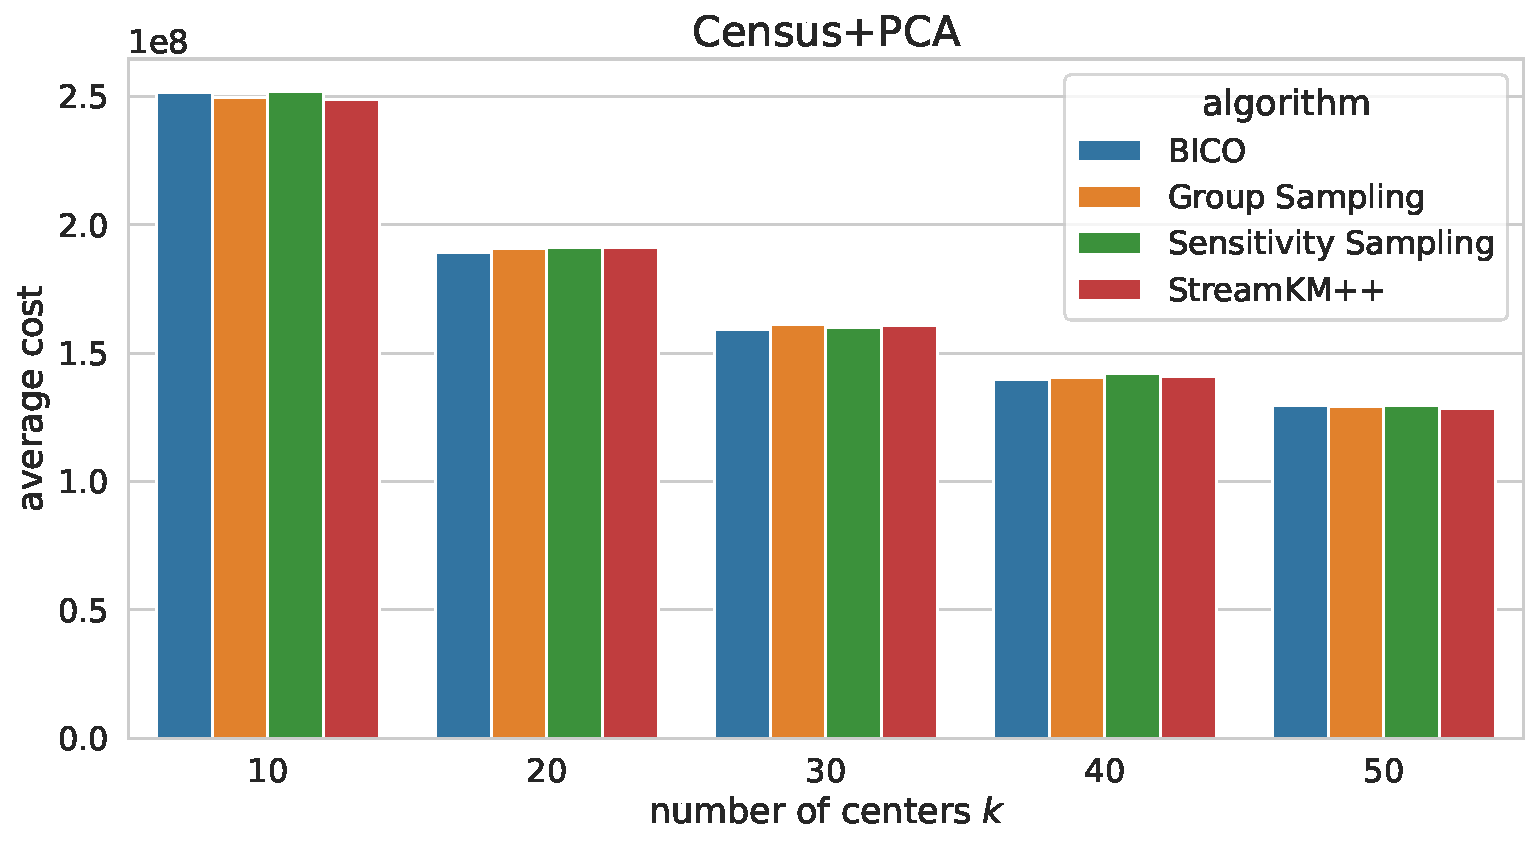
\includegraphics[width=.5\linewidth]{figures/costs-Census+PCA.pdf}
  }
  \newline \newline
  \label{fig:costs}
  \caption{The costs of the evaluated algorithms on \textit{Tower}, \textit{Covertype}, and \textit{Census} datasets.}
\end{figure*}


All four algorithms are equally matched when comparing them using the cost (see \cref{fig:costs}). For BICO and StreamKM++, the results are inline with 
Looking only at the costs for different values of $k$, we observe that all four algorithms are equally matched. 